\documentclass[10pt]{beamer}

\usepackage{appendixnumberbeamer}
\usepackage{booktabs}
\usepackage[scale=2]{ccicons}
\usepackage{pgfplots}
\usepackage{graphics}
\usepackage{braket}

\usepgfplotslibrary{dateplot}
\pdfstringdefDisableCommands{\def\translate#1{#1}}
\geometry{paperwidth=140mm, paperheight=105mm}
\usetheme{metropolis}
\bibliographystyle{abbrv}
\setbeamertemplate{frame footer}{ME738 - Special Topics in Materials}

\renewcommand{\footnotesize}{\fontsize{7pt}{8pt}\selectfont}

\title{Chip Scale Atomic Clocks Sources}
\subtitle{Working principles}
\date{March 20, 2024}
\author{Tommaso Bocchietti}
\institute{University of Waterloo}
\titlegraphic{\hfill
\includegraphics[height=1.5cm]{pdf/UniversityOfWaterloo_logo_horiz_pms.pdf}}

\begin{document}

\maketitle

\begin{frame}{Acronyms}
    \begin{description}
        \item[API] Application Programming Interface
        \item[LAN] Local Area Network
        \item[ASCII] American Standard Code for Information Interchange
    \end{description}
\end{frame}

\section{Toolbox}
% Light emission, ligth absorption, population inversion, stimulated emission

\begin{frame}{Energy quantization}

    \begin{columns}[c, onlytextwidth]

        \begin{column}{0.4\textwidth}

            Energy is a quantized quantity.

            The energy of a photon is given by the \textbf{Planck's relation}:

            \begin{equation}
                e = h f
            \end{equation}

            Unit of energy: electron-volt (eV) or Joule (J).

        \end{column}

        \begin{column}{0.6\textwidth}

            \begin{figure}
                \centering
                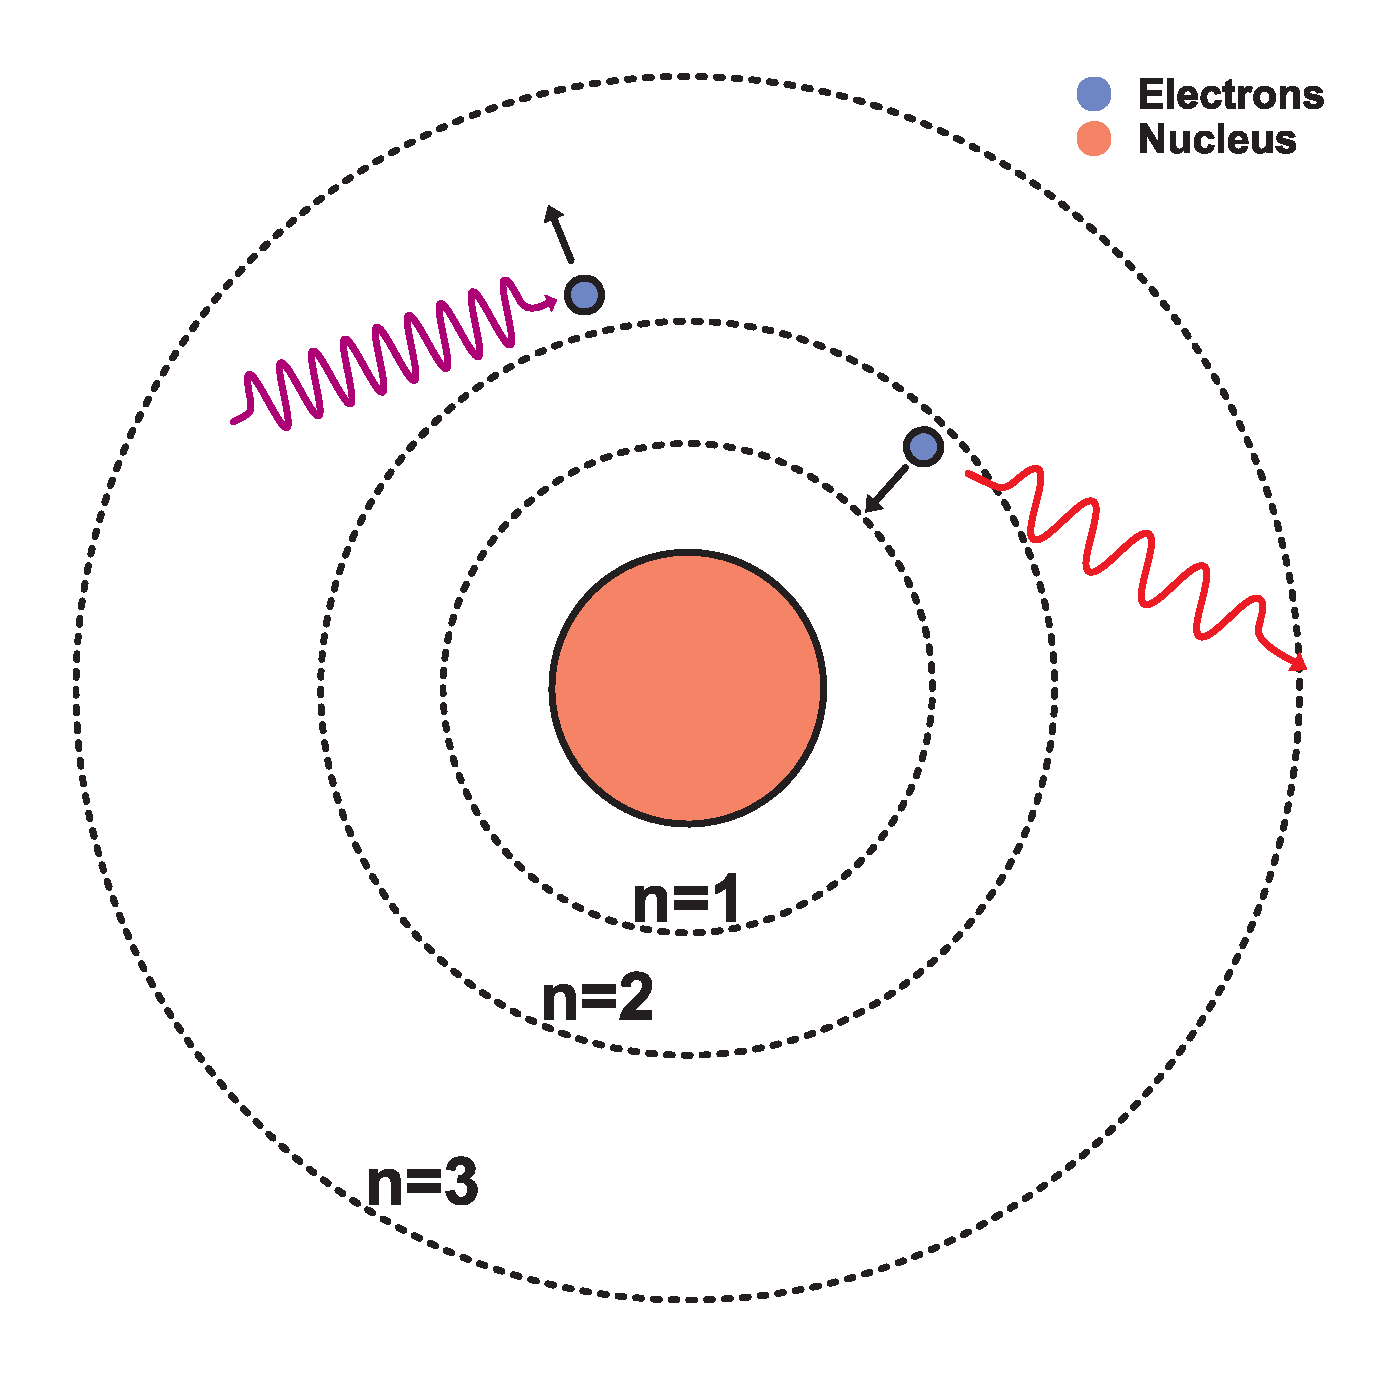
\includegraphics[width=0.9\textwidth]{pdf/eletronic-structure.pdf}
            \end{figure}

        \end{column}

    \end{columns}

    \begin{figure}[H]
        \centering

        \resizebox{\columnwidth}{!}{%
            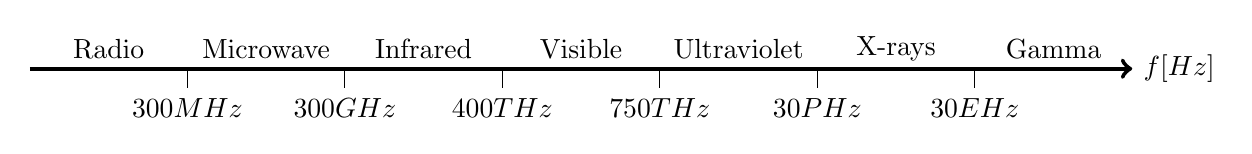
\begin{tikzpicture}[scale=0.5]
                % Spectrum lines
                \draw[ultra thick, ->] (0,0) -> (28,0) node[right] {$f \text{ [Hz]}$};

                % Wavelengths
                \foreach \w/\label in {4/$300MHz$, 8/$300GHz$, 12/$400THz$, 16/$750THz$, 20/$30PHz$, 24/$30EHz$}
                    {
                        \draw (\w,0) -- (\w,-0.5) node[below] {\label};
                    }

                % Labels
                \foreach \w/\label in {2/Radio, 6/Microwave, 10/Infrared, 14/Visible, 18/Ultraviolet, 22/X-rays, 26/Gamma}
                    {
                        \node at (\w, 0.5) {\label};
                    }

            \end{tikzpicture}
        }

    \end{figure}

\end{frame}



\begin{frame}{Rubidium and Cesium}

    We will deal with Rubidium (isotopes $^{85}Rb$ \& $^{87}Rb$) and Cesium ($^{133}Cs$).

    \begin{itemize}
        \item They are both alkali metals with a single valence electron.
        \item Their first ionization energy is low.
    \end{itemize}

    \begin{columns}[c, onlytextwidth]

        \begin{column}{0.5\textwidth}

            \begin{figure}
                \centering
                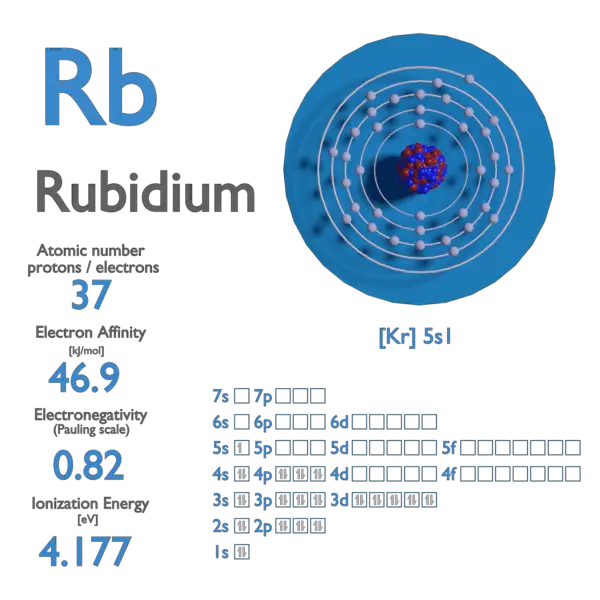
\includegraphics[width=0.8\textwidth]{img/Rubidium.png}
            \end{figure}

        \end{column}

        \begin{column}{0.5\textwidth}

            \begin{figure}
                \centering
                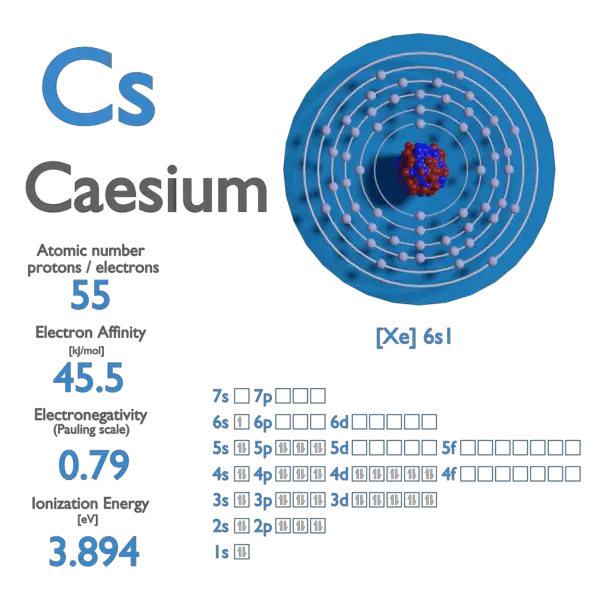
\includegraphics[width=0.8\textwidth]{img/Caesium.png}
            \end{figure}

        \end{column}

    \end{columns}

\end{frame}



\begin{frame}{Quantum levels}

    \begin{columns}[c, onlytextwidth]

        \begin{column}{0.45\textwidth}

            \begin{figure}
                \centering
                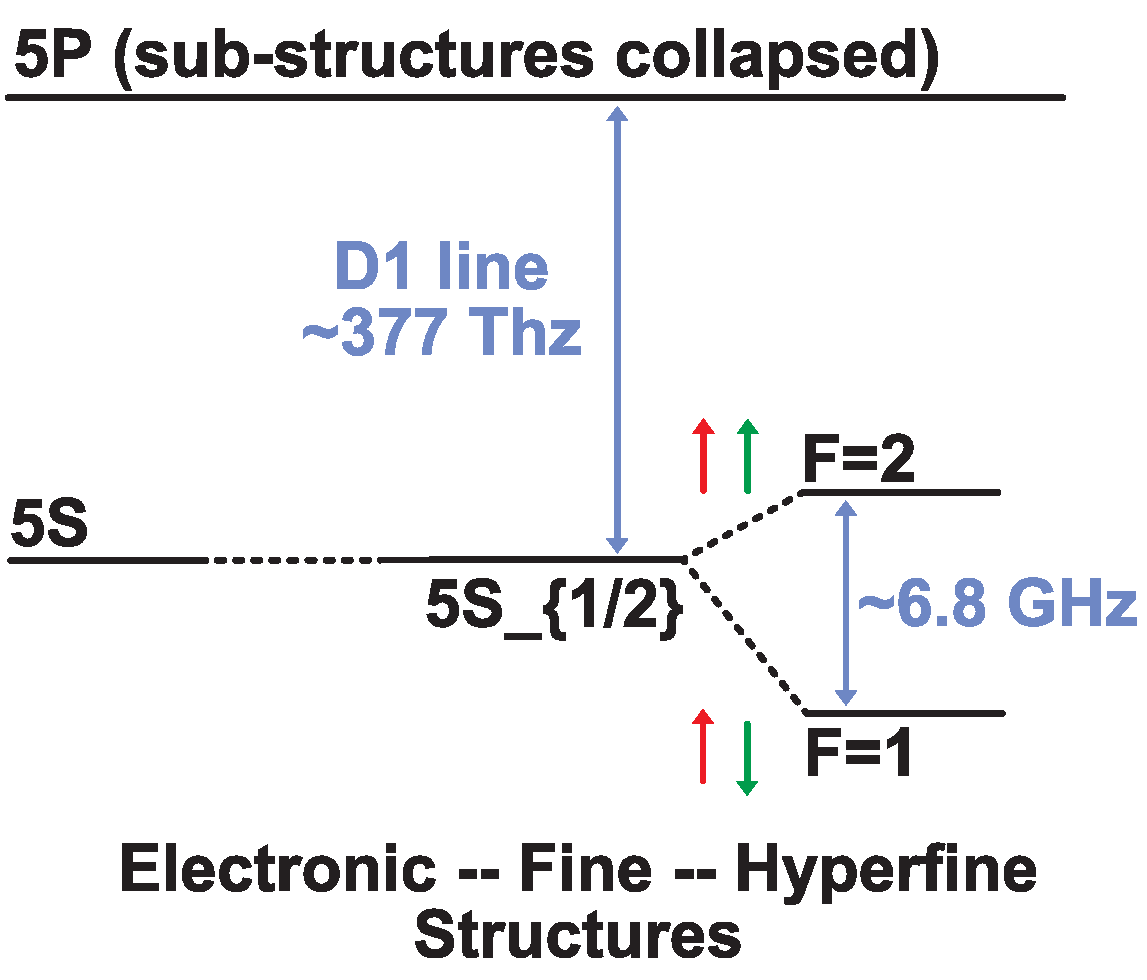
\includegraphics[width=0.8\textwidth]{pdf/structure-collapsed.pdf}
                \caption{$^{87}Rb$ quantum levels.}
            \end{figure}

        \end{column}

        \begin{column}{0.55\textwidth}

            \textbf{Elementary energy level ($n=1,2,3,\ldots$), can further be split.\footnotemark[1]}

            \vspace{10pt}

            Substructures are due to various quantum phenomena acting inside the atom domain.

            \begin{itemize}
                \item Electronic: classical orbital levels.
                \item Fine: electronic spin-orbit coupling.
                \item Hyperfine: \textcolor[HTML]{FF0000}{nuclear spin}-\textcolor[HTML]{00ED00}{electron spin} coupling.
            \end{itemize}

        \end{column}

    \end{columns}

    \vspace{10pt}

    \footnotetext[1]{For the purpose of the CSACs, we can consider the sub-$5P$ structures as collapsed into a single one.}

\end{frame}



% \begin{frame}{Optical pumping}
% \end{frame}
\section{CSAC Block Diagram}

\begin{frame}{Block diagram of a generic CSAC}

    \begin{figure}
        \centering
        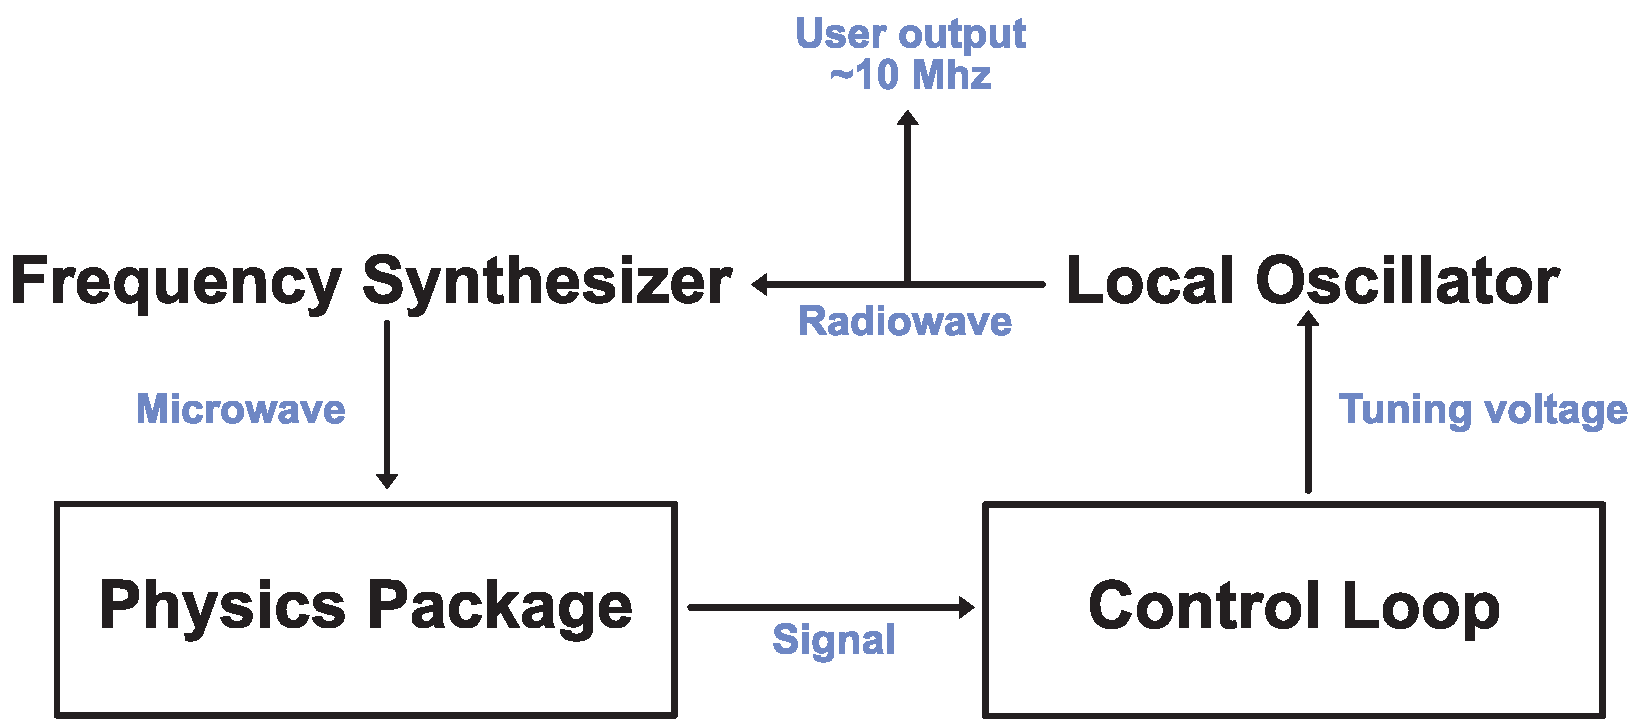
\includegraphics[width=0.8\textwidth]{pdf/logical-diagram.pdf}
    \end{figure}

    In the following slides, we are going to see:

    \begin{itemize}
        \item Physics Package
              \begin{itemize}
                  \item Based on Microwave Optical Double-Resonance (MODR)
                  \item Based on Coherent Population Trapping (CPT)
              \end{itemize}
        \item Control loop
        \item Local Oscillator
    \end{itemize}

\end{frame}
\section{Physics Package based on Microwave Optical Double-Resonance (MODR)}

\begin{frame}{$^{87}Rb$ Reference Cell}

    At the heart of a MODR based CSAC, we find a $^{87}Rb$ reference cell.

    \vspace{10pt}

    \begin{columns}[c, onlytextwidth]

        \begin{column}{0.45\textwidth}

            \begin{figure}
                \centering
                \only<1>{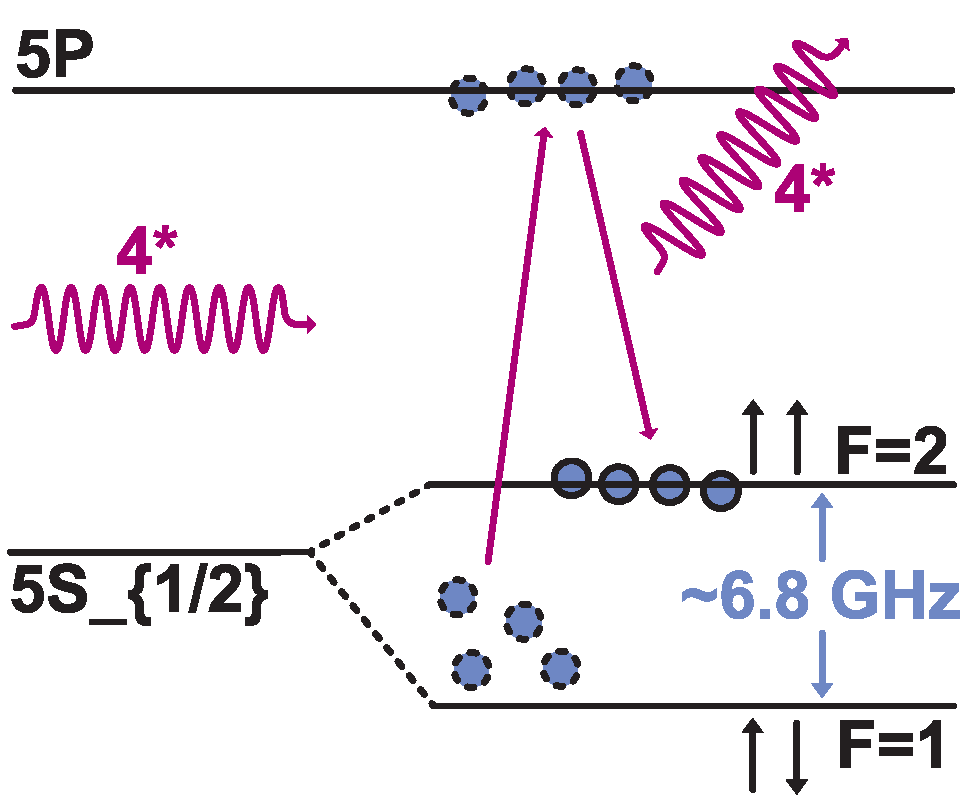
\includegraphics[width=0.9\textwidth]{pdf/MODR/01}}
                \only<2>{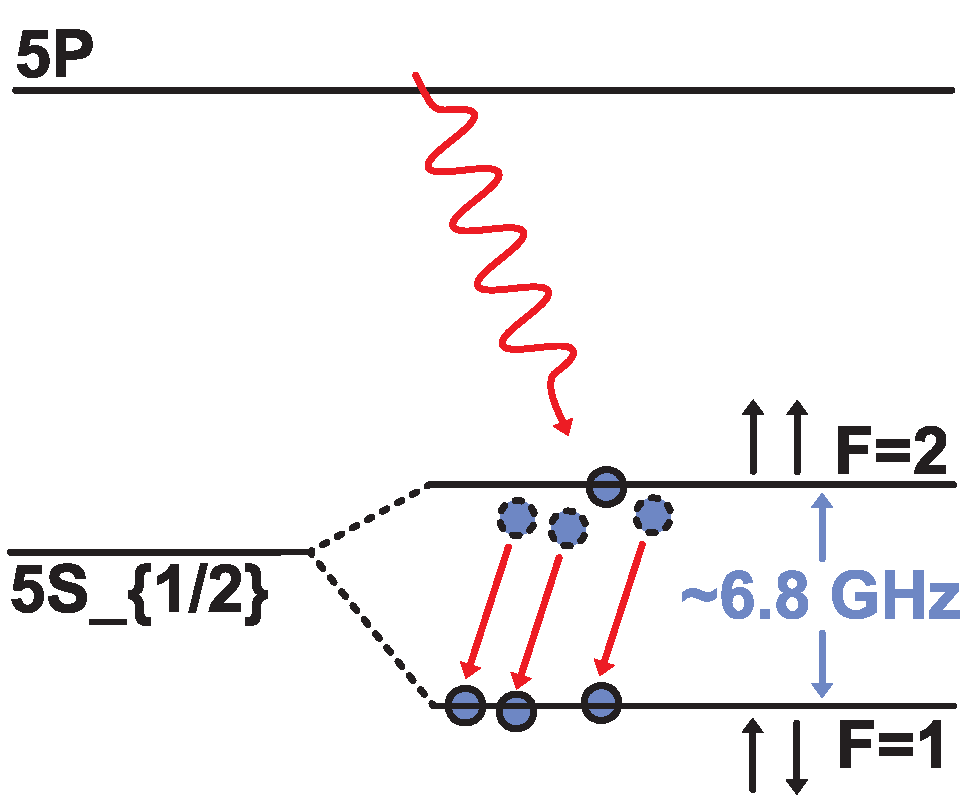
\includegraphics[width=0.9\textwidth]{pdf/MODR/02}}
                \only<3>{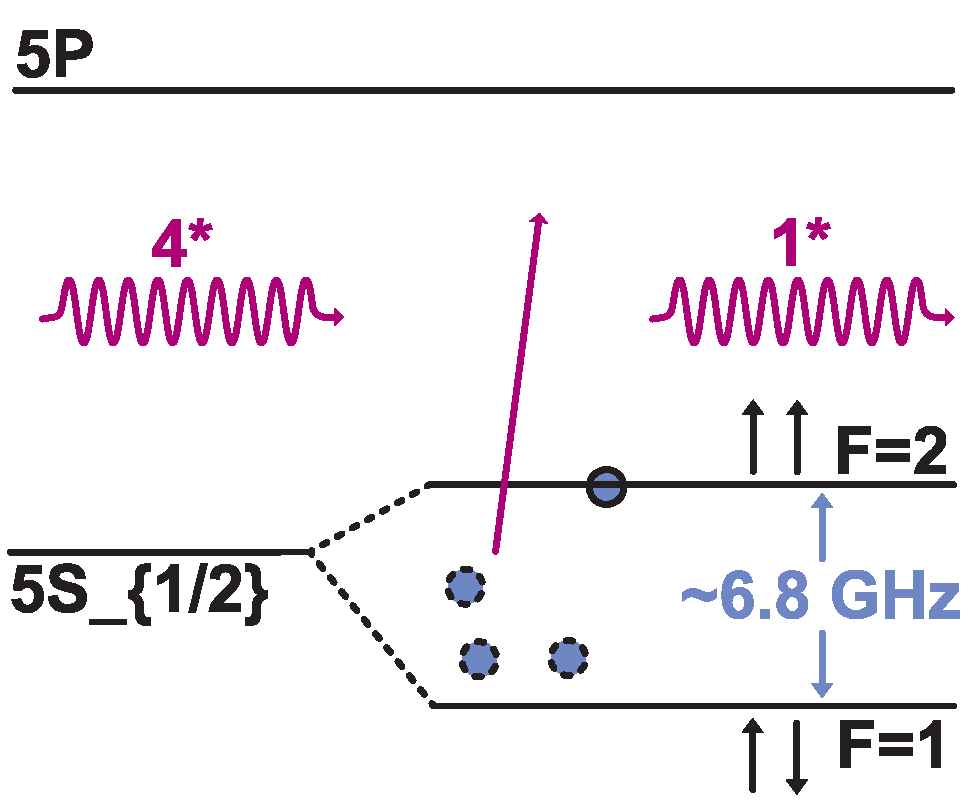
\includegraphics[width=0.9\textwidth]{pdf/MODR/03}}
            \end{figure}

        \end{column}

        \begin{column}{0.55\textwidth}

            We can distinguish 3 phases:

            \begin{enumerate}
                \item<1-> Optical Pumping (Population Inversion)
                \item<2-> Microwave Excitation
                \item<3-> Optical Pumping (Interrogation)
            \end{enumerate}

        \end{column}

    \end{columns}

    \vspace{10pt}

    \only<1>{Ground state population $F=\ket{1}$ gets pumped to $F=\ket{2}$.}
    \only<2>{Microwave tuned at the atomic resonance frequency ($\approx 6.8$ GHz) brings part of the population back to $F=\ket{1}$.}
    \only<3>{
        Depending on the intensity of the transmitted radiation, \textbf{we can infer if the microwave frequency was on resonance or not}.

        In this case, given that one photon was able to go through the cell, we can infer that the microwave frequency was not in resonance.
    }

\end{frame}



\begin{frame}{Photodetection}

    At the end of the cell, a photodiode is used to measure the intensity of the transmitted radiation.

    \begin{figure}
        \centering
        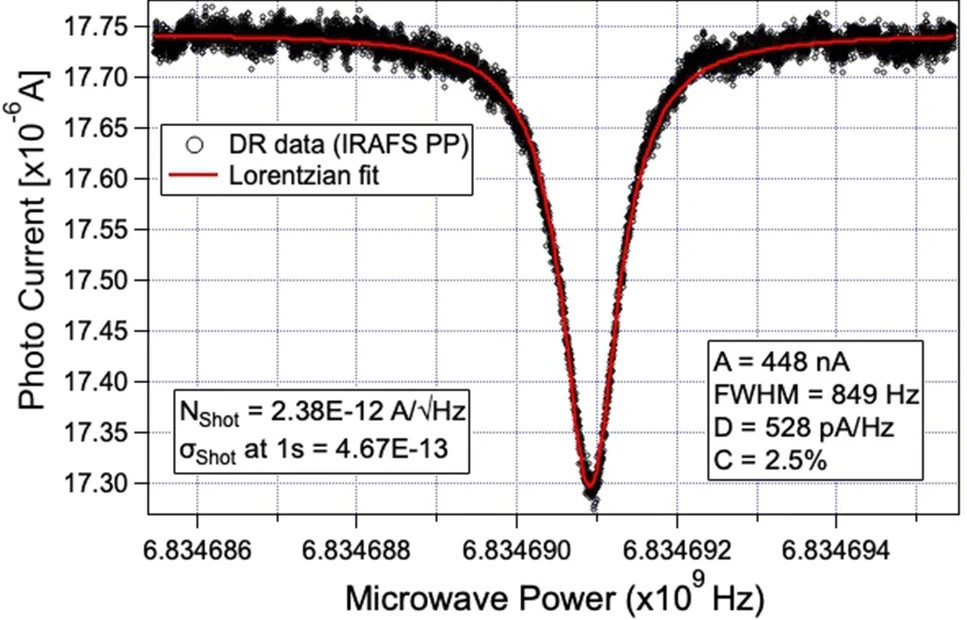
\includegraphics[width=0.7\textwidth]{img/Transmission}
    \end{figure}

    Our target is to stay at the dip of the transmission curve.

\end{frame}



\begin{frame}{Complete physics package for a MODR-based CSAC}

    % Previously analyzed components: \textit{Absorption Cell} and \textit{Photocell}.

    \begin{figure}
        \centering
        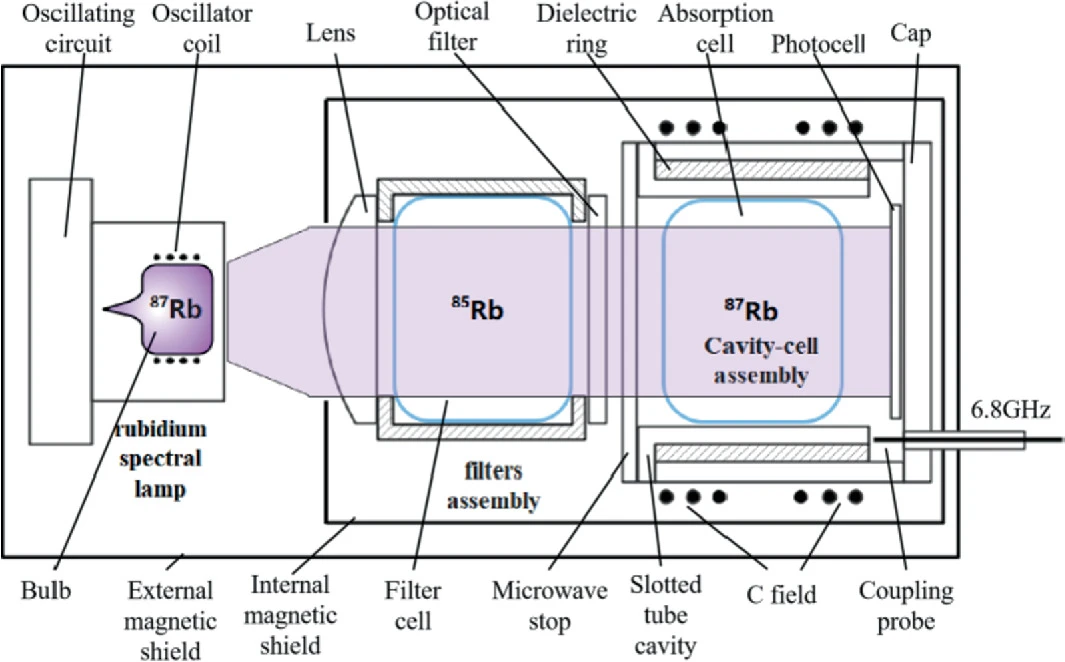
\includegraphics[width=0.7\textwidth]{img/Rubidium-Atomic-Clock-Physics-Package}
    \end{figure}

    Other notable components are:

    \begin{itemize}
        \item $^{87}Rb$ Bulb: high frequency radiation source.
        \item $^{85}Rb$ Filter cell: because of overlapping hyperfine levels, it filters out the unwanted transitions frequencies from the lamp.
        \item Microwave cavity: enhances the interaction between radiation and atoms.
    \end{itemize}

\end{frame}


\begin{frame}{Design bottleneck}

    \textit{...goal of developing an ultra-miniaturized, low-power, atomic time and frequency reference units...}

    \vspace{10pt}

    In case of a MODR-based CSAC, we can recognize multiple problematic areas:

    \begin{itemize}
        \item Power consumption: each component inside the physics package is usually oven controlled ($70\%$ of the total power consumption).
        \item Size: microwave cavity imposes a low limit ($L_{min} = \frac{c}{2f_{transition}} \approx 2.2cm$).
        \item Optical instabilities\footnotemark[1]: Stark shifts, Zeeman effects, internal wall gas collision.
    \end{itemize}

    \footnotetext[1]{More on this in the "Extra slides" section.}

\end{frame}


% \begin{frame}{Microwave Cavity}

%     The microwave cavity is used to enhance the interaction between the microwave radiation and the atoms.

%     \begin{figure}
%         \centering
%         \includegraphics[width=0.6\textwidth]{pdf/MODR/05}
%     \end{figure}

%     The cavity is tuned to the atomic resonance frequency.

% \end{frame}
\section{Physics Package based on Coherent Population Trapping (CPT)}
% CPT (Coherent Population Trapping) (theory -> physical components -> VCSEL


\section{Control loop}
% Control Loop (differences between the two, from where they start to where they close, freuqency for the various elements)

\begin{frame}{Control loop}

    \begin{columns}[c, onlytextwidth]

        \begin{column}{0.6\textwidth}

            \begin{figure}
                \centering
                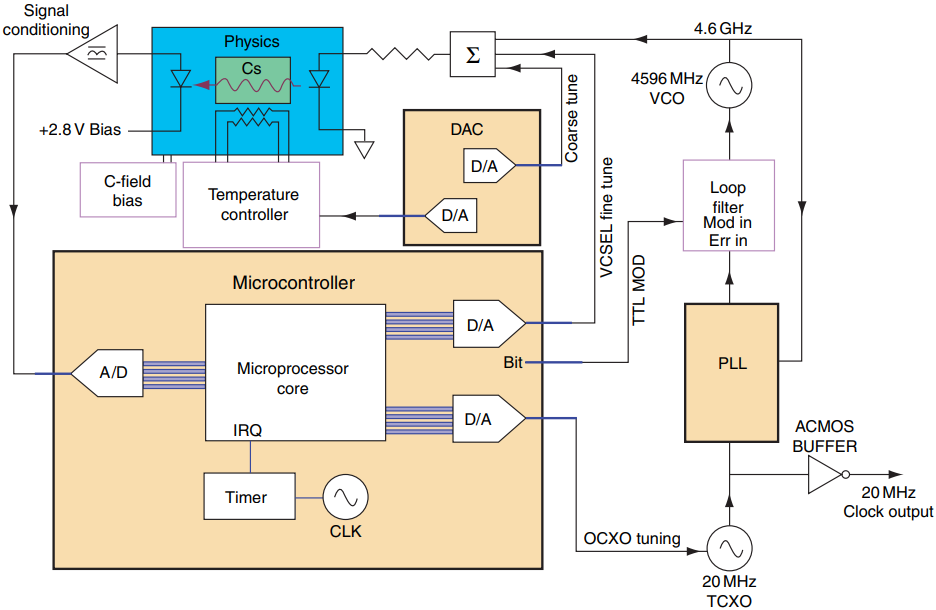
\includegraphics[width=0.9\textwidth]{img/Control-loop}
                \caption{Control loop block diagram.}
            \end{figure}

        \end{column}

        \begin{column}{0.4\textwidth}

            Close-loop control approach.
            Usually multiple PI controllers are used to operate a series of servo loops.

            \vspace{10pt}

            Indispensable targets:

            \begin{itemize}
                \item Laser temperature
                \item Cell temperature
                \item Laser frequency
                \item LO frequency
            \end{itemize}

        \end{column}

    \end{columns}

\end{frame}



\begin{frame}{Electronics}

    Here are some possible problematic areas:

    \begin{itemize}
        \item Stability in the voltage and current provided to VCO and VCSEL (highly sensitive components)
        \item Cross-talk between the various control loops
        \item Noise from the electronics
        \item Power consumption
    \end{itemize}

\end{frame}
\section{Local Oscillator}

\begin{frame}{Local Oscillator}

    Normally, the local oscillator in a CSAC is a quartz crystal oscillator (XO).

    There exist many versions of the XO, differentiated based on the environmental correction type applied to enhance stability:

    \begin{itemize}
        \item TCXO: Temperature Compensated Crystal Oscillator
        \item MCXO: Microcomputer Compensated Crystal Oscillator
        \item OCXO: Oven Controlled Crystal Oscillator
    \end{itemize}

\end{frame}



\begin{frame}{Quartz Crystal Oscillator}

    \textbf{At short time scales, the quartz crystal oscillator is the main source of instability} in a CSAC due to its phase noise.

    Here are some other problematic areas:

    \begin{itemize}
        \item High temperature sensitivity
        \item Power consumption (in case of temperature compensation or oven control)
        \item Aging and frequency drift
    \end{itemize}

    In the end, the choice of a local oscillator is a trade-off between stability and power consumption.

\end{frame}

\appendix

% \begin{frame}[standout]
    Extra slides
\end{frame}



\begin{frame}{$\mathrm{NO_x}$ Emissions}

    \begin{figure}[H]
        \centering
        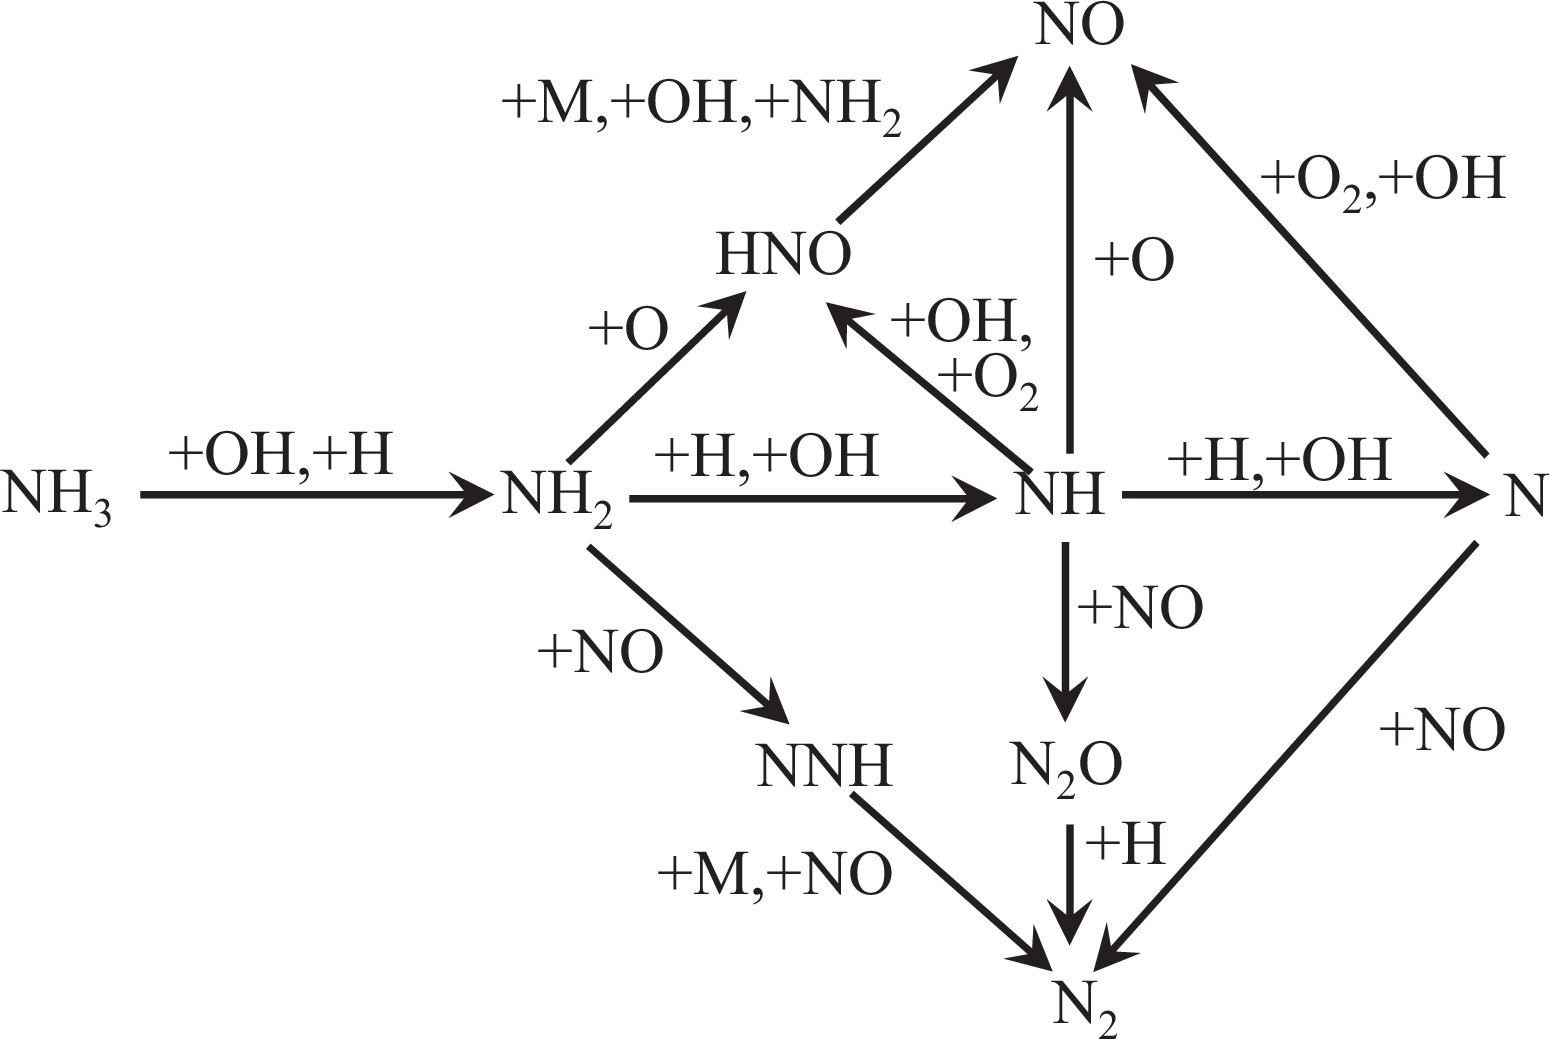
\includegraphics[width=0.6\textwidth]{img/NOx-emission-diagram.jpg}
        \caption{$\mathrm{NH_3}$ oxidation pathway}
    \end{figure}

\end{frame}



\begin{frame}

    More of the different types of NOx emissions

    More of the different types of fuel injectors

    Who uses a suitable replacing combution chamber, what's our target?

\end{frame}

\begin{frame}[allowframebreaks]{References}
    \nocite{*}
    \bibliography{references}
\end{frame}

\begin{frame}[standout]
    Questions?
\end{frame}

\begin{frame}[standout]
    Thank you!
\end{frame}

\end{document}